\documentclass{standalone}
\usepackage{tikz}

\usetikzlibrary{calc,math}


\begin{document}

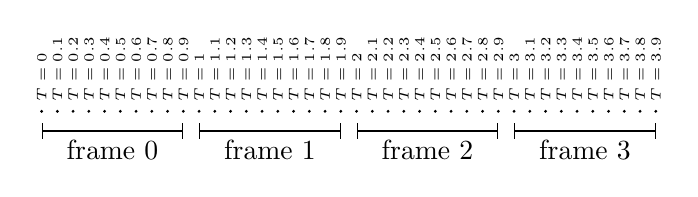
\begin{tikzpicture}
  \pgfkeys{/pgf/number format/.cd,fixed,precision=2}
  \foreach[evaluate={\i / 5} as \x,evaluate={\i / 10} as \t] \i in {0,...,39} {
    \draw (\x,0) circle [radius=0.01] node[right,rotate=90,font=\tiny] {$T=\pgfmathprintnumber{\t}$};
  }
  \foreach[evaluate={\i*2} as \x] \i in {0,...,3} {
    \draw[|-|] (\x,-0.25) -- ++(1.8,0) node[below,midway] {frame \i};
  }

\end{tikzpicture}

\end{document}